% --------------------------------------------------------------------------- %
\subsection{Функциональные структуры данных}
% --------------------------------------------------------------------------- %
\begin{frame}
    \begin{itemize}
        \item Были разработаны структуры данных, представляющие функции-предикаты, обработчики и селекторы.
    \end{itemize}

    \begin{figure}
        \smaller[1]
        \centering
        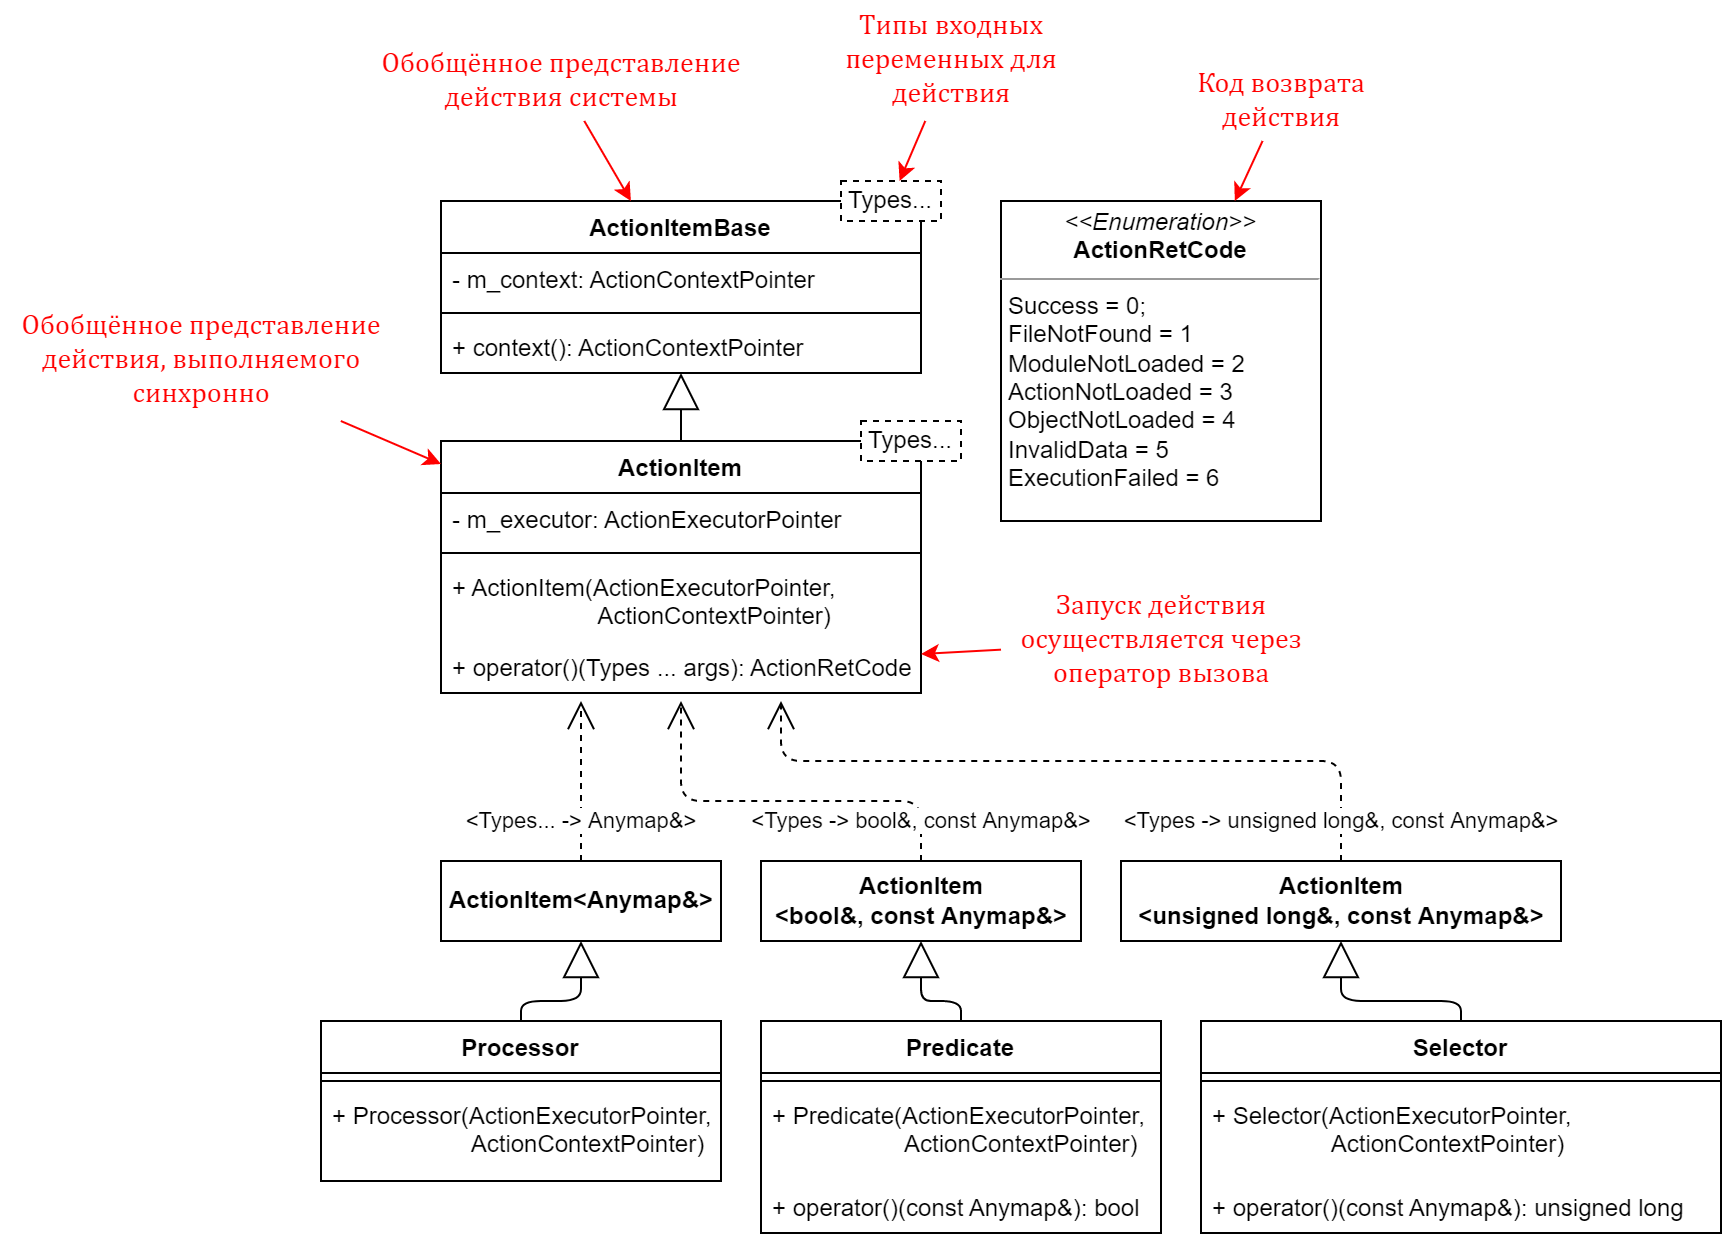
\includegraphics[height=0.67\textheight]{images/UML.graphFunctions.png}
        \caption{UML-диаграмма разработанных функциональных структур данных}
    \end{figure}

\end{frame}
% --------------------------------------------------------------------------- %
\subsection{Информационные структуры данных}
% --------------------------------------------------------------------------- %
\begin{frame}

\end{frame}
% --------------------------------------------------------------------------- %
\subsection{Требования к алгоритму обхода}
% --------------------------------------------------------------------------- %
\begin{frame}
    \begin{figure}
        \centering
        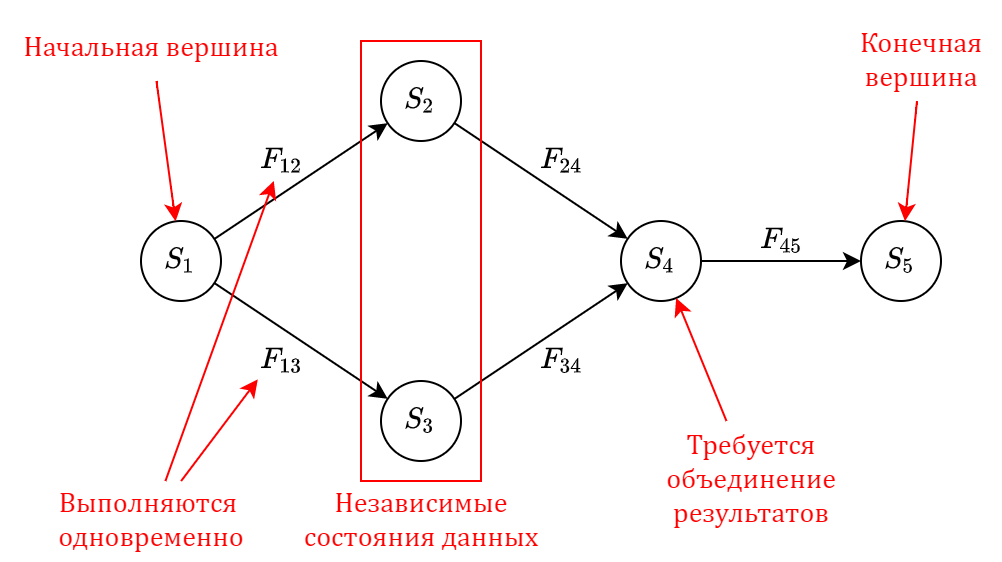
\includegraphics[width=0.6\textwidth]{images/illustration.parallel_run.png}
        \caption{Пример графовой модели, подразумевающей паралельный обход ветвей}
    \end{figure}

    Режим параллельного исполнения в вершине $S_1$ определяет, какие ресурсы будут задействованы для выполнения ветвей $S_1 \to S_2 \to S_4$ и $S_1 \to S_3 \to S_4$
\end{frame}

% --------------------------------------------------------------------------- %
\subsection{Управляющие структуры данных}
% --------------------------------------------------------------------------- %
\begin{frame}


\end{frame}
% --------------------------------------------------------------------------- %

